\section{Máximos e Mínimos para Funções de Duas Variáveis}

		\subsection{Definições \cite{morettin}}

		Uma importante aplicação do estudo das derivadas parciais é a otimização de funções. Otimizar uma função significa encontrar seu ponto de máximo ou de mínimo. Assim, determinar a máxima produção de um firma com um dado orçamento constitui um problema de maximização; entre possíveis combinações de insumos, aquela que nos permite obter certo nível de produção, a custo mínimo, consiste em resolver um problema de minimização. Vamos tornar mais precisas essas ideias, com algumas definições.

		Seja $f$ uma função de duas variáveis $x$ e $y$. Dizemos que um ponto $(x_{0}, y_{0})$ do domínio $D$ é um ponto de máximo relativo de $f$, ou simplesmente \textbf{ponto de máximo}, se existir uma bola aberta de centro $(x_{0}, y_{0})$ e raio $r$, tal que, para todo ponto $P(x, y)$ do domínio situado no interior dessa bola aberta, tenhamos

		\medskip

		$f(x, y) \leq f(x_{0}, y_{0})$

		\medskip

		[Lembre-se que $f(x, y) = z$, logo estamos trabalhando com uma bola aberta de centro $(x_{0}, y_{0})$ e raio $r$ no plano $xOy$].

		\medskip

		Ao número $f(x_{0}, y_{0})$ damos o nome de valor máximo de $f$ (Figura 11.1).

		\begin{figure}[H]
				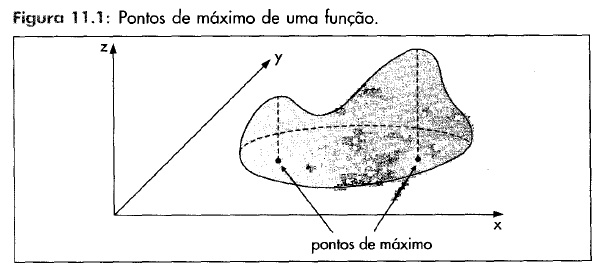
\includegraphics[height=6.5cm]{images/morettin_figura-11-1}
		\end{figure}

		Analogamente, dizemos que um ponto $(x_{0}, y_{0})$ do domínio $D$ é um ponto de mínimo relativo de $f$, ou simplesmente \textbf{ponto de mínimo}, se existir uma bola aberta de centro $(x_{0}, y_{0})$ e raio $r$, tal que, para todo ponto $P(x, y)$ do domínio situado no interior dessa bola aberta de centro $(x_{0}, y_{0})$ e raio $r$, tal que, para todo ponto $P(x, y)$ do domínio situado no interior dessa bola aberta, tenhamos

		\medskip

		$f(x, y) \geq f(x_{0}, y_{0})$ .

		\medskip

		Ao número $f(x_{0}, y_{0})$ damos o nome de valor mínimo de $f$ (Figura 11.2).

		\begin{figure}[H]
				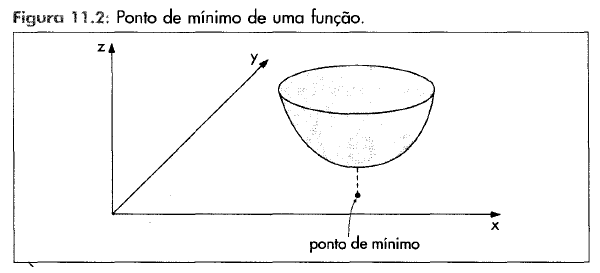
\includegraphics[height=6.5cm]{images/morettin_figura-11-2}
		\end{figure}

		Seja $f$ um função de duas variáveis $x$ e $y$. Dizemos que um ponto $(x_{0}, y_{0})$ do domínio $D$ é um ponto de \textbf{máximo global (ou absoluto)} de $f$ se, para todo ponto $P(x, y)$ do domínio tivermos

		\medskip

		$f(x, y) \leq f(x_{0}, y_{0})$ .

		\medskip

		Analogamente, dizemos que um ponto $(x_{0}, y_{0})$ do domínio $D$ é um ponto de \textbf{mínimo global (ou absoluto)} de $f$ se, para todo ponto $P(x, y)$ do domínio, tivermos

		\medskip

		$f(x, y) \geq f(x_{0}, y_{0})$ .

		\medskip

		A descoberta de um ponto de máximo ou de mínimo exige, na maioria dos casos, o conhecimento do gráfico de $f$, o que, conforme vimos, não é um problema fácil.

		Entretanto, existem teoremas que nos auxiliam nesse sentido, e que passaremos a estudar.

		\bigskip

		\textbf{Teorema 11.1} \cite{morettin}

		\medskip

		Seja $f$ uma função com duas variáveis $x$ e $y$ e seja $(x_{0}, y_{0})$ um ponto interior ao domínio.
		Se $(x_{0}, y_{0})$ for um ponto de máximo ou de mínimo de $f$ e se existirem derivadas parciais $fx$ e $fy$, então

		\medskip

		$fx(x_{0}, y_{0}) = 0$ \ e \ $fy(x_{0}, y_{0}) = 0$ .

		\bigskip

		\textbf{Demonstração}

		\medskip

		Suponhamos que $(x_{0}, y_{0})$ seja um ponto de máximo. Existe a bola aberta de centro $(x_{0}, y_{0})$ e raio $r$, no interior do domínio $D$, cujos pontos $(x, y)$ são tais que $f(x, y) \leq f(x_{0}, y_{0})$ (Figura 11.3).

		\begin{figure}[H]
				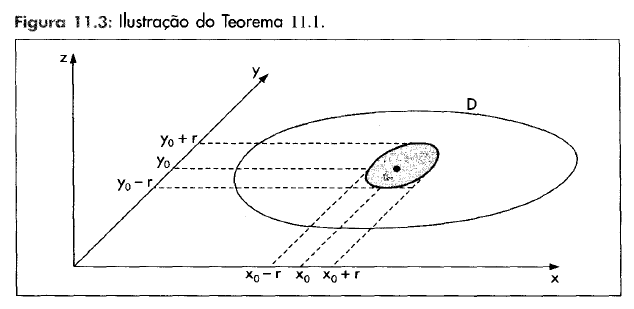
\includegraphics[height=6.5cm]{images/morettin_figura-11-3}
		\end{figure}

		Consideremos os pontos dessa bola para os quais $y = y_{0}$. Então $f(x, y_{0})$ será função somente de $x$. Mas, como $f(x, y_{0}) \leq f(x_{0}, y_{0})$ para $x_{0} - r < x < x_{0} + r$, segue-se que a função $f(x, y_{0})$ de uma variável tem um ponto de máximo em $(x_{0}, y_{0})$ e, consequentemente, $fx(x_{0}, y_{0}) = 0$.

		Analogamente, se considerarmos os pontos da bola aberta para os quais $x = x_{0}$, então $f(x_{0}, y)$ será só função de $y$. Mas, como $f(x_{0}, y) \leq f(x_{0}, y_{0})$ para $y_{0} - r < y < y_{0} + r$, segue-se que a função $f(x_{0}, y)$, de uma variável, tem um ponto máximo em $(x_{0}, y_{0})$ e, consequentemente $fy(x_{0}, y_{0}) = 0$.

		Em resumo, \textbf{se $\boldsymbol{(x_{0}, y_{0})}$ for ponto de máximo, então $\boldsymbol{fx(x_{0}, y_{0}) = 0}$ \ e \ $\boldsymbol{fy(x_{0}, y_{0}) = 0}$}.

		Os pontos que anulam simultaneamente as derivadas parciais $fx$ e $fy$ são chamados \textbf{pontos críticos de $f$}.

		\bigskip

		\textbf{Observações}

		\medskip

		Antes de prosseguirmos, cumpre salientarmos algumas considerações bastante importantes em tudo que segue.

		\begin{enumerate}[label=(\roman*)]

			\item O Teorema não nos garante a existência de pontos de máximo ou de mínimo, mas sim \textbf{possíveis [candidatos] pontos de máximo ou mínimo}. Assim, pode ocorrer de termos $fx(x_{0}, y_{0}) = 0$ \ e \ $fy(x_{0}, y_{0}) = 0$ sem que $(x_{0}, y_{0})$ seja ponto de máximo ou mínimo.

			Um exemplo desse fato é o da função $f(x, y) = xy$, em que $fx = y$ e $fy = x$; o ponto crítico é $(0, 0)$.

			Assim, se tomarmos uma bola aberta de centro $(0, 0)$ e raio $r$, teremos:

			\begin{enumerate}[label=\alph*)]

				\item para os pontos dessa bola aberta situados no interior do primeiro e terceiro quadrantes, $f(x, y) = xy > 0$, pois $x$ e $y$ têm o mesmo sinal;

				\item para os pontos dessa bola aberta situados no interior do segundo e quarto quadrantes $f(x, y) = xy < 0$, pois $x$ e $y$ têm sinais contrários.

			\end{enumerate}

			Logo

			\medskip

			$(0,0)$ não é ponto de máximo nem de mínimo.

			\medskip

			Verifica-se que o gráfico dessa função tem o aspecto de uma $sela de cavalo$. O ponto $(0, 0)$ é chamado de \textbf{ponto de sela} (Figura 11.4).

			\begin{figure}[H]
				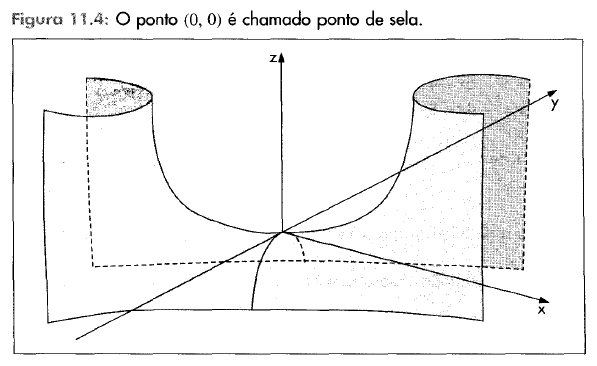
\includegraphics[height=7cm]{images/morettin_figura-11-4}
			\end{figure}

			\begin{figure}[H]
				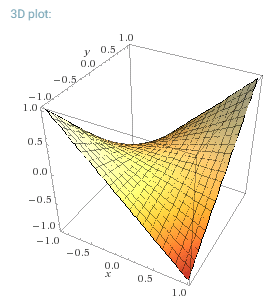
\includegraphics[height=7cm]{images/wolframalpha_figura-1-1}
				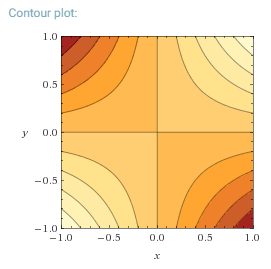
\includegraphics[height=7cm]{images/wolframalpha_figura-1-2} \cite{wolframalpha}
			\end{figure}

			De um modo geral, todo ponto crítico $(x_{0}, y_{0})$ que não é de máximo nem de mínimo é chamado ponto de sela.

			Encontramos um problema semelhante com qualquer plano horizontal em $xOz$. Planos horizontais não têm um único ponto de máximo ou de mínimo, pois qualquer ponto pode ser considerado máximo e mínimo ao mesmo tempo $f(x, y) = f (x_{0}, y_{0})$.

			\item O Teorema só se aplica a pontos interiores do domínio. Assim, os pontos que anulam as derivadas parciais $fx$ e $fy$ só podem ser pontos de máximo ou mínimo do interior do domínio. A análise dos pontos de fronteira deve ser feita à parte, como veremos a seguir.

		\end{enumerate}

	\subsection{Critérios para Identificação de Pontos de Máximo ou Mínimo \cite{morettin}}

		O Teorema 11.1 permitiu-nos determinar os possíveis pontos de máximo ou de mínimo no interior do domínio, sem, contudo, identificá-los. O Teorema 11.2, que veremos a seguir, permitirá esta identificação. Sua demonstração poderá ser vista, por exemplo, em Leithold (1977).

		\bigskip

		\textbf{Teorema 11.2} \cite{morettin}

		\medskip

		Seja $f$ uma função de duas variáveis $x$ e $y$, contínua, com derivadas parciais até segunda ordem contínuas. Seja $(x_{0}, y_{0})$ um ponto crítico de $f$. Chamemos o determinante

		\medskip

		$
		H(x_{0}, y_{0}) =
		\begin{vmatrix}

			fxx(x_{0}, y_{0}) & fxy(x_{0}, y_{0}) \\
			fyx(x_{0}, y_{0}) & fyy(x_{0}, y_{0})

		\end{vmatrix}
		$

		\medskip

		de Hessiano ($H$) (em homenagem ao matemático alemão Ludwig Otto Hesse, 1811-1874) de $f$ no ponto $(x_{0}, y_{0})$. Se:

		\begin{enumerate}[label=(\alph*)]

			\item $H(x_{0}, y_{0}) > 0$ e $fxx(x_{0}, y_{0}) < 0$, então $(x_{0}, y_{0})$ será ponto de máximo de $f$,

			\item $H(x_{0}, y_{0}) > 0$ e $fxx(x_{0}, y_{0}) > 0$, então $(x_{0}, y_{0})$ será ponto de mínimo de $f$,

			\item $H(x_{0}, y_{0}) > 0$, então $(x_{0}, y_{0})$ será ponto de sela de $f$.

		\end{enumerate}
		
	\subsection{Uma Aplicação: Ajuste de Retas pelo Método dos Mínimos Quadrados \cite{morettin}}
	
	\subsection{Análise dos Pontos de Fronteira \cite{morettin}}

		Até agora, vimos como encontrar máximos e mínimos de funções analisando apenas os pontos interiores ao domínio (pois os teoremas dados só se aplicam a esses pontos). A análise dos pontos de fronteira (quando existem) terá que ser feita sem o auxílio destes teoremas. Uma das formas usadas para abordar tais situações é por meio das curvas de nível da função a ser otimizada. Os exemplos esclarecerão este tipo de abordagem.

		\bigskip

		\textbf{Exemplo}. Consideremos a função $f$ dada por $f(x, y) = 2x + y$, definida no domínio $D$ dado pelas inequações

		\medskip

		$x \geq 0$, \\
		$y \geq 0$, \\
		$x + y \leq 7$.

		\begin{enumerate}[label=\alph*)]

			\item Em primeiro lugar, notemos que o conjunto $D$ é constituído pela reunião do triângulo da Figura 11.9 com sua parte interna. A fronteira do domínio é constituída dos lados $\overline{AB}$, $\overline{BC}$ e $\overline{AC}$.

			\begin{figure}[H]
				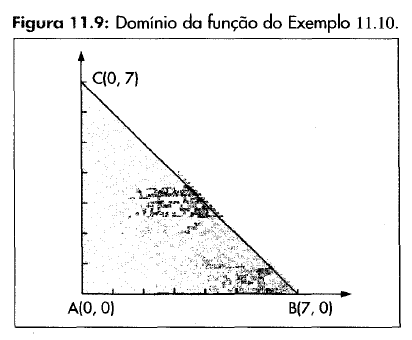
\includegraphics[height=7cm]{images/morettin_figura-11-9}
			\end{figure}

			\item A função $f(x, y) = 2x + y$ admite como curvas de nível o feixe de paralelas à reta $2x + y = 0$, pois qualquer curva de nível $c$ tem por equação a reta $2x + y = c$, que é paralela à $2x + y = 0$ qualquer que seja $c$.

			Eis algumas curvas de nível. Seus gráficos comparecem na Figura 11.10:

			\medskip

			$c = 1 \rightarrow 2x + y = 1$ \\
			$c = 2 \rightarrow 2x + y = 2$ \\
			$c = 3 \rightarrow 2x + y = 3$ .

			\begin{figure}[H]
				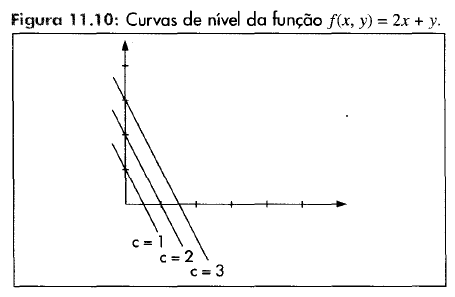
\includegraphics[height=6cm]{images/morettin_figura-11-10}
			\end{figure}

			\begin{figure}[H]
				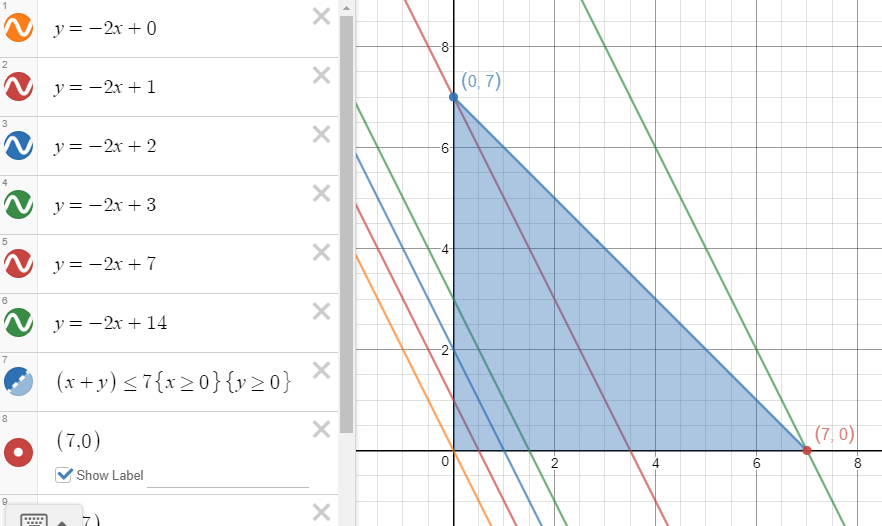
\includegraphics[height=7cm]{images/desmos_figura-1} \cite{desmos}
			\end{figure}

			Notemos, nesse exemplo, que, quanto mais a reta se distancia da origem, maior é o valor de $c$.

			\item Como todos os pontos $(x, y)$ da curva de nível $c$ produzem um valor constante para $f(x, y)$, o ponto da curva de maior nível que intercepta $D$ é o ponto de máximo de $f$; no caso do exemplo em questão, tal ponto é $B(7, 0)$. A curva de menor nível que intercepta $D$ é o ponto de mínimo de $f$; no caso, tal ponto é $A(0, 0)$ (Figura 11.11).

			\begin{figure}[H]
				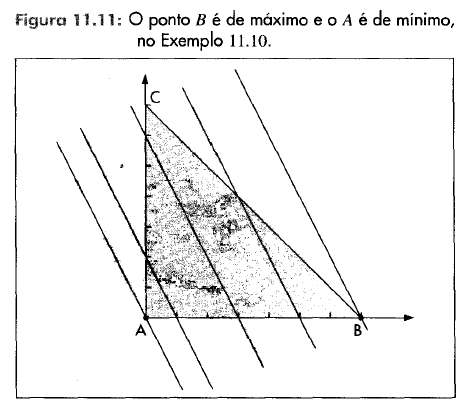
\includegraphics[height=8cm]{images/morettin_figura-11-11}
			\end{figure}

			\item O ponto $(0, 0)$ é o ponto de mínimo absoluto e $(7, 0)$ é o ponto de máximo absoluto de $f$.

			\item Entre os pontos interiores a $D$, não existem pontos de máximo ou mínimo, pois as derivadas parciais nunca se anulam ($fx = 2$ e $fy = 1$).

		\end{enumerate}

		É intuitivo perceber, nesse exemplo, que os pontos de máximo ou mínimo estão nos vértices do triângulo. Assim, por simples inspeção do valor de $f$ nos pontos $A$, $B$ e $C$, poderíamos descobrir os pontos de máximo e mínimo.
			De fato,

		\medskip

		$f(x, y) = 2x + y$, \\
		$A(0, 0) \rightarrow f(0, 0) = 2 \times 0 + 0 = 0$, \\
		$B(7, 0) \rightarrow f(7, 0) = 2 \times 7 + 0 = 14$, \\
		$C(0, 7) \rightarrow f(0, 7) = 2 \times 0 + 7 = 7$,

		\medskip

		e, portanto, $A(0, 0)$ é o ponto de mínimo e $B(7, 0)$ é o ponto de máximo de $f$.

		\bigskip

		\textbf{Exemplo}. Consideremos a função dada por $f(x, y) = x + y$, definida no domínio $D$ determinado pelas inequações

		\medskip

		$x \geq 0$, \\
		$y \geq 0$, \\
		$2x + y \geq 10$, \\
		$x + 2y \geq 10$.

		\medskip

		\begin{enumerate}[label=\alph*)]

			\item O conjunto $D$ é formado pelos pontos da região indicada na Figura 11.12.

			\begin{figure}[H]
				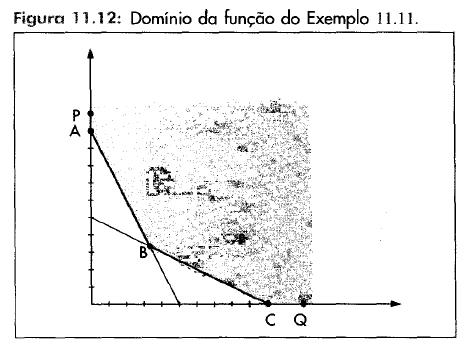
\includegraphics[height=7cm]{images/morettin_figura-11-12}
			\end{figure}

			Os pontos $A$, $B$ e $C$ têm coordenadas $(0, 10)$, $\left( \cfrac{10}{3}, \cfrac{10}{3} \right)$ e $(10, 0)$ respectivamente; o ponto $B$ é a intersecção das retas $2x + y = 10$ e $x + 2y = 10$.

			Os pontos de fronteira do domínio são aqueles dos segmentos $\overline{AB}$ e $\overline{BC}$, bem como os das semi-retas, $\overline{AP}$ e $\overline{CQ}$.

			\item A função $f(x, y) = x + y$ admite como curvas de nível o feixe de retas paralelas à reta $x + y = 0$.

			Eis algumas curvas de nível e seus respectivos gráficos (Figura 11.13):

			\medskip

			$c = 1 \rightarrow x + y = 1$ \\
			$c = 2 \rightarrow x + y = 2$ \\
			$c = 3 \rightarrow x + y = 3$ \\

			\begin{figure}[H]
				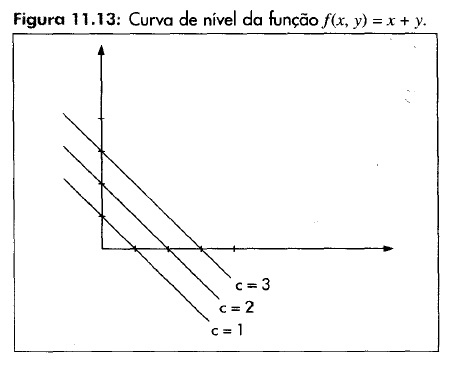
\includegraphics[height=7cm]{images/morettin_figura-11-13}
			\end{figure}

			\item O ponto de mínimo de $f$ é o ponto da curva de menor nível que intercepta $D$. Assim, o ponto de mínimo é o ponto $B\left( \cfrac{10}{3}, \cfrac{10}{3} \right)$ (Figura 11.14).

			\begin{figure}[H]
				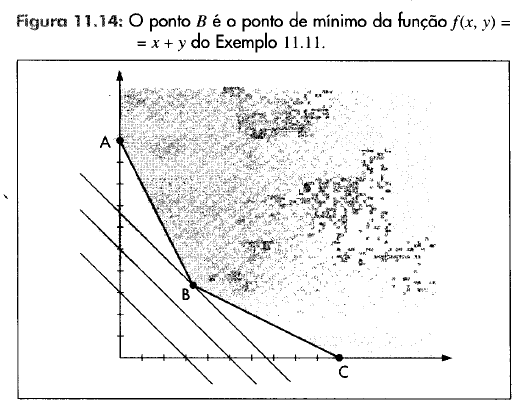
\includegraphics[height=8cm]{images/morettin_figura-11-14}
			\end{figure}

			\item A função $f$ não tem ponto de máximo em $D$, pois não existe curva de maior nível de $f$ que intercepte $D$ (Figura 11.15).

			\begin{figure}[H]
				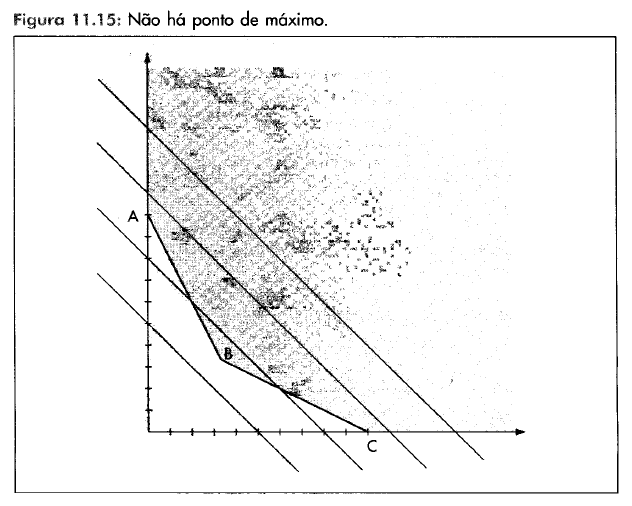
\includegraphics[height=9cm]{images/morettin_figura-11-15}
			\end{figure}

		\end{enumerate}

		\textbf{Exemplo}. Consideremos a função dada por $f(x, y) = x + y$ e domínio $D$ determinado pelas inequações

		\medskip

		$x \geq 0$, \\
		$y \geq 0$, \\
		$x + y \leq 3$.

		\medskip

		\begin{enumerate}[label=\alph*)]

			\item O conjunto $D$ é constituído pela região triangular da Figura 11.16. Os vértices do triângulo são $A(0, 0)$, $B(3, 0)$ e $C(0, 3)$.

			\begin{figure}[H]
				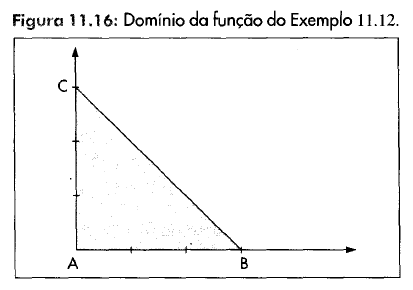
\includegraphics[height=6cm]{images/morettin_figura-11-16}
			\end{figure}

			\item A função dada admite como curvas de nível o feixe de paralelas à reta $x + y = 0$ (Figura 11.17).

			\item Todos os pontos do segmento $\overline{BC}$ são pontos de máximo, pois a reta determinada por $\overline{BC}$ tem o mesmo coeficiente angular que o feixe de paralelas $(-1)$. O ponto de mínimo de $f$ é o ponto $A(0, 0)$ (Figura 11.18).

			\begin{figure}[H]
				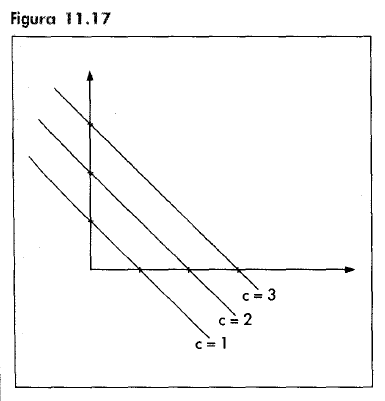
\includegraphics[height=7cm]{images/morettin_figura-11-17}
				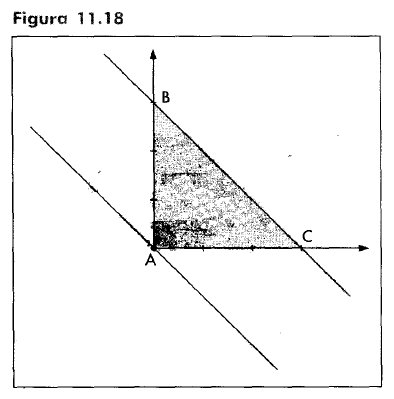
\includegraphics[height=7cm]{images/morettin_figura-11-18}
			\end{figure}

		\end{enumerate}

		\textbf{Exemplo}. Determine o ponto de máximo e mínimo da função $f(x, y) = x + y$ no domínio dado por $D = \{(x, y) \in \mathbb{R} \mid x^{2} + y^{2} \leq 1\}$.

		\medskip

		O domínio da função é o círculo de centro na origem e raio $1$ (Figura 11.19).

		As curvas de nível da função são as retas do feixe de paralelas $x + y = c$ (Figura 11.20).

		Portanto, os pontos de máximo e de mínimo são os pontos de tangência de $x + y = c$ com a circunferência $x^{2} + y^{2} = 1$ (Figura 11.21).

		\begin{figure}[H]
			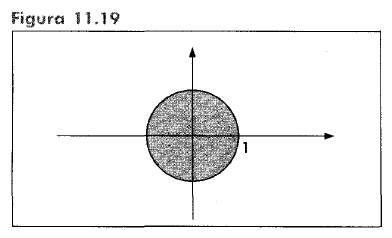
\includegraphics[height=5cm]{images/morettin_figura-11-19}
			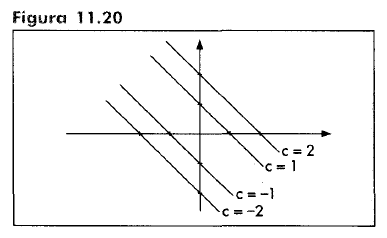
\includegraphics[height=5cm]{images/morettin_figura-11-20}
			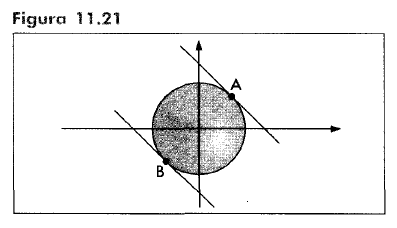
\includegraphics[height=5cm]{images/morettin_figura-11-21}
		\end{figure}

		Assim sendo, devemos impor que o sistemas de equações

		\bigskip

		$
		\begin{cases}
			x + y = c & (11.1)\\
			x^{2} + y^{2} = 1 & (11.2)
		\end{cases}
		$

		\bigskip

		tenha solução única.

		\medskip

		De (11.1) temos $y = c - x$. Substituindo em (11.2), teremos:

		\medskip

		$2x^{2} - 2cx + c^{2} - 1 = 0$ \ \ (11.3)

		\medskip

		Para que (11.3) tenha uma única raiz, seu discriminante ($\Delta$) deve ser nula. Assim:

		\medskip

		$\Delta = 4c^{2} - 8(c^{2} -1) = -4c^{2} + 8 = 0 \implies c = \sqrt{2} \ \text{ou} \ c = - \sqrt{2}$

		\medskip

		É evidente que para $c = \sqrt{2}$ teremos um ponto de máximo e para $c = - \sqrt{2}$ teremos um ponto de mínimo.

		Para $c = \sqrt{2}$ a equação (11.3) fica igual a $2x^{2} - 2\sqrt{2}x + 1 = 0$, cuja raiz é $x = \cfrac{\sqrt{2}}{2}$.

		O valor de $y$ é dado pela equação (11.1), isto é: $y = \sqrt{2} - \cfrac{\sqrt{2}}{2} = \cfrac{\sqrt{2}}{2}$. Portanto o ponto de máximo é $\left( \cfrac{\sqrt{2}}{2}, \cfrac{\sqrt{2}}{2} \right)$.

		Para $c = - \sqrt{2}$ concluímos de modo análogo que o ponto de mínimo é $\left( - \cfrac{\sqrt{2}}{2}, - \cfrac{\sqrt{2}}{2} \right)$.
		
	\subsection{Máximos e Mínimos Condicionados \cite{morettin}}
	
		\subsubsection{Método da Substituição \cite{morettin}}

		\subsubsection{Método dos Multiplicadores de Lagrange \cite{morettin}}